\section{Background}
\label{sec:background}
\subsection{Wheeled Platforms and Motion Constraints}
A wheeled mobile robot moves through driven or steered rolling contacts whose footprint, arrangement, and contact conditions constrain the paths it can execute. Differential-drive robots turn by varying the left and right wheel speeds, skid-steer robots use the same actuation with lateral slip at the contacts, Ackermann vehicles steer the front wheels with a finite minimum turning radius, and omnidirectional platforms generate lateral motion through their wheel arrangement. For a planar reference point with position $(x,y)$ and heading $\psi$, a common idealization is
\begin{equation}
\dot{x}=v\cos\psi,\qquad \dot{y}=v\sin\psi,\qquad \dot{\psi}=\omega,
\label{eq:unicycle}
\end{equation}
where $v$ is longitudinal speed and $\omega$ is angular speed. Under pure rolling, a differential-drive robot with wheel radius $r$, track width $b$, and right and left wheel angular speeds $\omega_R$ and $\omega_L$ satisfies
\begin{equation}
v=\frac{r}{2}(\omega_R+\omega_L),\qquad
\omega=\frac{r}{b}(\omega_R-\omega_L).
\label{eq:differential}
\end{equation}
An ideal bicycle approximation for Ackermann steering instead gives
\begin{equation}
\omega=\frac{v}{L}\tan\delta,
\label{eq:ackermann}
\end{equation}
where $L$ is the wheelbase and $\delta$ is the steering angle. Slip violates the pure-rolling assumption, wheel calibration affects odometry, and steering and acceleration limits constrain tracking. On uneven ground, suspension, pitch, roll, clearance, traction, and payload further affect feasibility, which means that a planar collision-free path may be physically unsuitable even when localization is accurate.

\subsection{The Navigation Stack and Its Degradation}
Fig.~\ref{fig:stack} shows the principal functions of a navigation system, the points at which degradation enters, and the interfaces examined in Section~\ref{sec:challenges}. Cameras, color and depth (RGB-D) cameras, LiDAR, radar, inertial measurement units (IMUs), wheel encoders, global navigation satellite system (GNSS) receivers, and ultra-wideband (UWB) ranging supply measurements with calibration parameters and timestamps. The estimator infers robot state from these measurements and motion inputs, the mapping algorithm estimates spatial structure, the planner selects a route or trajectory, and the controller converts that reference into actuator commands. A supervisor can interrupt execution when measurements, models, or resources no longer support the current action. Deployed systems realize these functions through interacting maps, planners, controllers, and recovery behaviors, for example in a robot operating system (ROS) navigation stack with planner fallback~\cite{P_S16} or under behavior-tree supervision~\cite{P_N17}.

\begin{figure*}[t]
\centering
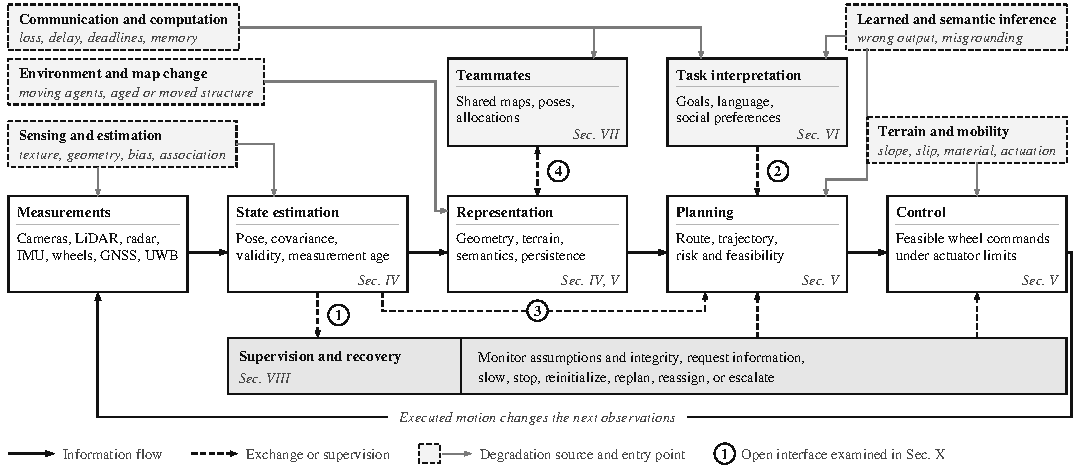
\includegraphics[width=\textwidth]{figures/fig-stack.pdf}
\caption{Navigation functions, degradation entry points, and open interfaces. Each function is colored by the section that reviews it. Teammates and task interpretation supply information to the motion stack rather than bypassing vehicle constraints, and the numbered markers locate the four interfaces of Section~X.}
\label{fig:stack}
\end{figure*}

An estimator can be described through the posterior
\begin{equation}
p(\mathbf{x}_t,\mathcal{M}\mid\mathbf{z}_{1:t},\mathbf{u}_{1:t}),
\label{eq:belief}
\end{equation}
where $\mathbf{x}_t$ is the robot state, $\mathcal{M}$ is the map, and $\mathbf{z}_{1:t}$ and $\mathbf{u}_{1:t}$ denote observation and motion-input sequences available through time $t$. Localization estimates state relative to a given reference, whereas SLAM estimates state and map jointly, commonly through visual--inertial odometry (VIO) or LiDAR--inertial odometry (LIO). ORB-SLAM3~\cite{B_ORBSLAM32021} and FAST-LIO2~\cite{B_FASTLIO22022} are representative visual and LiDAR--inertial systems on which several reviewed methods build. Loop closures constrain revisited places, and an incorrect association can introduce correlated errors into many states. Downstream decisions may therefore require the covariance, association confidence, and age of an estimate as well as its mean. Geometric, topological, and semantic representations retain different information, and a representation sufficient for one decision can be insufficient for another. A place graph may support a long route while omitting a small obstacle, and a terrain label may describe appearance without establishing traction for a loaded vehicle.

In local planning, the dynamic window approach (DWA) searches admissible velocity commands, timed-elastic-band (TEB) optimization adjusts a sequence of poses and timing variables, and model predictive control (MPC) repeatedly solves a finite-horizon control problem. DWA and TEB remain common comparators in recent evaluations~\cite{P_M06,P_M30}. A controller using a control barrier function (CBF) constrains inputs to keep the state within an admissible set under stated assumptions~\cite{P_E24,P_E26}. For a control-affine model $\dot{\mathbf{x}}=f(\mathbf{x})+g(\mathbf{x})\mathbf{u}$, a common condition is
\begin{equation}
\nabla h(\mathbf{x})^{\mathsf T}\bigl[f(\mathbf{x})+g(\mathbf{x})\mathbf{u}\bigr]
+\alpha(h(\mathbf{x}))\geq 0,
\label{eq:cbf}
\end{equation}
where $f$ denotes the drift dynamics, $g$ maps the control input $\mathbf{u}$ to the state derivative, $h(\mathbf{x})\geq0$ defines the admissible set, and $\alpha$ is a suitable increasing function with $\alpha(0)=0$. The resulting safety argument depends on the state information, dynamics, admissible inputs, and update implementation, and penalizing a barrier violation in an objective does not establish the condition during execution.

Here, \emph{degradation} denotes an operating change that reduces the quality or validity of the information, models, resources, or physical capabilities required for navigation. Fig.~\ref{fig:stack} distinguishes four sources that can occur within one episode. Sensing and estimation degradation includes weak texture, illumination change, poorly constrained scan geometry, GNSS denial, timing errors, and incorrect associations, and many measurements may still carry little information along one motion direction. Terrain and mobility degradation includes slopes, vegetation, soft ground, slip, and changed actuator behavior, where similar geometry can hide different friction or sinkage. Environment and map change includes moving people, altered layouts, and construction, which requires the robot to separate transient obstacles from lasting map updates. Communication and computation degradation includes packet loss, partitions, stale shared states, delayed model responses, and missed deadlines, and a restored link raises the further problem of reconciling states accumulated during the outage.

\subsection{Accuracy, Task Performance, and Integrity}
Absolute trajectory error (ATE) measures differences between estimated and reference poses after a declared alignment, relative pose error (RPE) measures motion error over a declared interval, and both are commonly summarized by the root mean square error (RMSE). Their values depend on alignment freedoms, scale treatment, synchronization, aggregation, and the dependence of the reference on the evaluated sensors. Task measures include goal success, collisions, interventions, completion time, coverage, and energy, while success weighted by path length (SPL) combines goal success with path efficiency. Neither task success nor low ATE identifies the source of a failure or the ability to recover after an alarm.

Integrity concerns the risk of an unacceptable estimation error without an adequate warning. A useful conceptual statement is
\begin{equation}
\Pr\!\left(E_t>A_t\ \land\ \text{no timely alert at }t\right),
\label{eq:integrity}
\end{equation}
where $E_t$ is an error magnitude and $A_t$ is an application-specific alert limit. A protection level is an error bound associated with a specified integrity model, and a covariance alone is not a calibrated protection level. Particle-filter and SLAM integrity analyses account for fault hypotheses and association errors when relating alarm conditions to hazardous error~\cite{P_M28,P_X07}. For navigation, the warning must also reach a response policy early enough for the motion and stopping constraints of the robot.

\subsection{Datasets, Simulators, and Transfer}
Table~\ref{tab:benchmarks} relates representative resources to the evidence they can support. M2DGR and M2UD provide ground-robot sequences with sensing and motion difficulties and real-time kinematic (RTK) references~\cite{P_M41,P_F11}, GEODE and HK-MEMS extend the comparison to varied degeneracy and sensor conditions~\cite{P_S33,P_S21}, and robot/network simulation supports repeated reception and control conditions~\cite{P_F13}. Recorded data support reproducible estimator comparisons, although replay does not change future measurements when a planner acts differently. A closed-loop simulator supplies that feedback under its model, whereas hardware adds physical interaction and execution timing, and the three settings answer different causal questions.

\begin{table*}[t]
\centering
\caption{Representative evaluation resources, their intended uses, and relevant limitations.}
\label{tab:benchmarks}
\surveytableformat
\begin{tabularx}{\linewidth}{@{}L{2.8cm}L{5.4cm}Y@{}}
\toprule
\textbf{Resource} & \textbf{Evaluation use} & \textbf{Relevant limitation} \\
\midrule
M2DGR~\cite{P_M41} & Ground-robot localization across everyday sensing and motion difficulties & Estimation errors must be connected separately to task outcomes \\
\addlinespace[3pt]
M2UD~\cite{P_F11} & Uneven-terrain localization/mapping and runtime-aware comparison & References mix RTK and offline SLAM, external checks cover selected routes, and mapping includes handheld capture \\
\addlinespace[3pt]
GEODE~\cite{P_S33} & Degeneracy comparisons across sensor conditions & Sensor-specific coverage and severity affect comparisons, and replay does not test action-dependent recovery \\
\addlinespace[3pt]
HK-MEMS~\cite{P_S21} & Multi-sensor localization and reference comparisons & Missing reference intervals and failed trajectories require explicit coverage reporting \\
\addlinespace[3pt]
Robot/network simulation~\cite{P_F13} & Designed reception and control conditions with repeated trials & A network-in-the-loop simulation is distinct from a distributed physical deployment \\
\bottomrule
\end{tabularx}
\end{table*}
